% Options for packages loaded elsewhere
\PassOptionsToPackage{unicode}{hyperref}
\PassOptionsToPackage{hyphens}{url}
%
\documentclass[
]{book}
\usepackage{amsmath,amssymb}
\usepackage{lmodern}
\usepackage{iftex}
\ifPDFTeX
  \usepackage[T1]{fontenc}
  \usepackage[utf8]{inputenc}
  \usepackage{textcomp} % provide euro and other symbols
\else % if luatex or xetex
  \usepackage{unicode-math}
  \defaultfontfeatures{Scale=MatchLowercase}
  \defaultfontfeatures[\rmfamily]{Ligatures=TeX,Scale=1}
\fi
% Use upquote if available, for straight quotes in verbatim environments
\IfFileExists{upquote.sty}{\usepackage{upquote}}{}
\IfFileExists{microtype.sty}{% use microtype if available
  \usepackage[]{microtype}
  \UseMicrotypeSet[protrusion]{basicmath} % disable protrusion for tt fonts
}{}
\makeatletter
\@ifundefined{KOMAClassName}{% if non-KOMA class
  \IfFileExists{parskip.sty}{%
    \usepackage{parskip}
  }{% else
    \setlength{\parindent}{0pt}
    \setlength{\parskip}{6pt plus 2pt minus 1pt}}
}{% if KOMA class
  \KOMAoptions{parskip=half}}
\makeatother
\usepackage{xcolor}
\usepackage{longtable,booktabs,array}
\usepackage{calc} % for calculating minipage widths
% Correct order of tables after \paragraph or \subparagraph
\usepackage{etoolbox}
\makeatletter
\patchcmd\longtable{\par}{\if@noskipsec\mbox{}\fi\par}{}{}
\makeatother
% Allow footnotes in longtable head/foot
\IfFileExists{footnotehyper.sty}{\usepackage{footnotehyper}}{\usepackage{footnote}}
\makesavenoteenv{longtable}
\usepackage{graphicx}
\makeatletter
\def\maxwidth{\ifdim\Gin@nat@width>\linewidth\linewidth\else\Gin@nat@width\fi}
\def\maxheight{\ifdim\Gin@nat@height>\textheight\textheight\else\Gin@nat@height\fi}
\makeatother
% Scale images if necessary, so that they will not overflow the page
% margins by default, and it is still possible to overwrite the defaults
% using explicit options in \includegraphics[width, height, ...]{}
\setkeys{Gin}{width=\maxwidth,height=\maxheight,keepaspectratio}
% Set default figure placement to htbp
\makeatletter
\def\fps@figure{htbp}
\makeatother
\setlength{\emergencystretch}{3em} % prevent overfull lines
\providecommand{\tightlist}{%
  \setlength{\itemsep}{0pt}\setlength{\parskip}{0pt}}
\setcounter{secnumdepth}{5}
\usepackage{booktabs}
\usepackage{amsthm}
\usepackage[T1]{fontenc}
\usepackage[utf8]{inputenc}
\usepackage{lmodern}
\usepackage[brazil]{babel}
\usepackage[left=3cm,right=2cm,top=2cm,bottom=2cm]{geometry}
\makeatletter
\def\thm@space@setup{%
  \thm@preskip=8pt plus 2pt minus 4pt
  \thm@postskip=\thm@preskip
}
\makeatother
\ifLuaTeX
  \usepackage{selnolig}  % disable illegal ligatures
\fi
\usepackage[]{natbib}
\bibliographystyle{apalike}
\IfFileExists{bookmark.sty}{\usepackage{bookmark}}{\usepackage{hyperref}}
\IfFileExists{xurl.sty}{\usepackage{xurl}}{} % add URL line breaks if available
\urlstyle{same} % disable monospaced font for URLs
\hypersetup{
  pdftitle={Estatística + R},
  pdfauthor={Ana Paula Fernandes},
  hidelinks,
  pdfcreator={LaTeX via pandoc}}

\title{Estatística + R}
\author{Ana Paula Fernandes}
\date{2023-04-25}

\begin{document}
\maketitle

{
\setcounter{tocdepth}{1}
\tableofcontents
}
\hypertarget{bem-vindos}{%
\chapter{Bem-vindos!}\label{bem-vindos}}

\begin{figure}
\centering
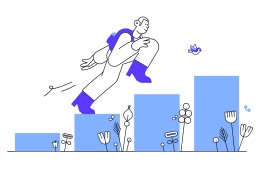
\includegraphics{pablita-stepping-up.png}
\caption{ Fonte: \url{http://icons8.com}}
\end{figure}

Esse livro \emph{online} tem como propósito principal de ser um guia para as aulas de estatística, referente as disciplinas de \textbf{Bioestatística} para os curso de Medicina e Educação Física e \textbf{Estatística Aplicada} para o curso de Psicologia da Universidade Federal do Triangulo Mineiro (UFTM) \url{http://www.uftm.edu.br}. E como objetivo secundário, ser uma referência de consulta para todos os discentes que passaram por essas disciplinas, bem como, para todos que estão interessados em realizar análises de dados por meio da linguagem R e o ambiente de desenvolvimento RStudio.

Sugestões, correções ou qualquer outra forma de interação são sempre bem-vindas! Então, por favor, não hesite em me escrever \href{mailto:anapaula.fernandes@uftm.edu.br}{\nolinkurl{anapaula.fernandes@uftm.edu.br}}.

E vamos lá!

\hypertarget{intro}{%
\chapter{Introdução}\label{intro}}

Ao longo de algum tempo ministrando aulas de estatísticas conclui que estudar estatística com auxílio de recursos computacionais é bem mais eficaz, quero dizer, é mais fácil entender os conceitos téoricos, lidar com recusos visuais (gráficos) e, de fato, transformar o contéudo estudado na disciplina em uma ferramenta para pesquisas científicas, quando se trata de analisar dados.

Ministrando aulas para os cursos da área de saúde e esporte sempre ouvi dos discentes que estatística é matemática, e sempre digo que estatística é estatística! É normal alguns discentes não assimilarem, em princípio, a importância da disciplina na grade do seu curso, e realmente, alguns acham até que é assunto que deveria ficar restrito aos curso das exatas. Assim, a primeira tarefa é desconstruir essa ideia.

A estatística é \textbf{MULTIDICIPLINAR}, ela está em tudo na verdade\ldots{} e para dizer uma coisa ``bem chique'' a estatística é a base da Inteligência Artificial. Advinha quem está por trás dos famosos algortimos das redes sociais? Ou das sugestões de filmes que aparecem no seu \emph{streamming} favorito? Ou no ranque de busca realzada no \emph{Google}?

E sendo um pouco mais ``acadêmica'', dentro do nosso propósito:

Qualquer competição ou treinamento esportivo está recheado de estatística, como medir o desempenho de um time ou atleta? Veja esse exemplo aqui:

Na medicina, estudos epidemiologicos, e claro, da medicina baseada em evidências, tem o suporte da estatística. Veja esse exemplo aqui:

Exemplo da psicologia\ldots{} Veja esse exemplo aqui:

Basta realizar uma busca com os termos estatística e um campo do seu curso que você se interessa, que você encontrará um artigo científico. E se você não encontrar, comece a escreve sobre o tema!

Quando olhamos os artigos acima, podemos ver que todos eles tem resultados \textbf{descritivos} e \textbf{inferenciais}.

\hypertarget{atividade}{%
\section{Atividade}\label{atividade}}

\textbf{1. Busque um artigo do campo de seu interesse que utiliza a estatística.}

\begin{itemize}
\item
  Qual é o principal objetivo da pesquisa?
\item
  Como a pesquisa foi realizada?
\item
  Observe o que é descrito por meio de tabelas ou gráficos.
\item
  Faça uma lista de termos que são relacionados à estatística.
\end{itemize}

\textbf{Sugestão}

\begin{quote}
Periódicos da área da Ciência dos Esportes
\end{quote}

\begin{quote}
Periódicos da área de Medicina
\end{quote}

\begin{quote}
Periódicos da área de Piscologia
\end{quote}

\hypertarget{definiuxe7uxf5es-iniciais}{%
\chapter{Definições iniciais}\label{definiuxe7uxf5es-iniciais}}

\begin{quote}
A estatística é divida em duas partes
\end{quote}

\begin{itemize}
\item
  Estatística DESCRITIVA
\item
  Estatística INFERENCIAL
\end{itemize}

\begin{quote}
Essas duas partes são conectadas pela téoria de probabilidade, especificamente pelas distribuições de probabilidade.
\end{quote}

\begin{quote}
População x Amostra
\end{quote}

\begin{itemize}
\item
  POPULAÇÃO
\item
  AMOSTRA
\end{itemize}

\hypertarget{tamanho-da-amostra}{%
\chapter{Tamanho da amostra}\label{tamanho-da-amostra}}

O cálculo do tamanho da amostra é um procedimento simples, porém ele depende de vários conceitos da parte da estatística inferencial, e também dos objetivos das análises que serão feitas na pesquisa. Essa resposta está aqui \{\#tamanho-amostra\}.

\hypertarget{atividade-1}{%
\section{Atividade}\label{atividade-1}}

\textbf{2. Responda a partir do artigo buscado na atividade 1.}

\begin{itemize}
\item
  O autores mencionaram sobre o cálculo do tamanho da amostra?
\item
  A população da pesquisa foi bem delineada (bem definida)?
\item
  Os autores mencionaram se a pesquisa foi submetida ao Comitê de Ética.
\item
  Qual a importância de submeter a pesquisa ao Comitê de Ética?
\end{itemize}

\textbf{Importante}

\begin{quote}
Conheça o Comitê de Ética em Pesquisa (CEP) da UFTM
\end{quote}

\url{https://www.uftm.edu.br/comitesecomissoes/cep}

\hypertarget{ambiente-computacional}{%
\chapter{Ambiente computacional}\label{ambiente-computacional}}

Existem vários softwares que são dedicados a análise estatística que vão do maravilhoso SPSS (da IMB) às planilhas eletrônicas (como o Excel). Para citar alguns algumas dessas ferramentas:

\textbf{Softwares pagos}

\begin{itemize}
\item
  SPSS \url{https://www.ibm.com/br-pt/spss}
\item
  Stata \url{https://www.stata-brasil.com/software/stata.html}
\item
  SAS \url{https://www.sas.com/pt_br}
\item
  JMP \url{https://www.jmp.com/}
\item
  Prisma \url{https://software.com.br/p/prism}
\item
  Minitab \url{https://osbsoftware.com.br/produto/minitab-statistical-software}
\item
  Excel (Microsoft)
\end{itemize}

\textbf{Softwares livre}

\begin{itemize}
\item
  Jamovi \url{https://www.jamovi.org}
\item
  OpenStat \url{https://openstat.info}
\end{itemize}

\textbf{Liguagens computacionais}

\begin{itemize}
\item
  R \url{https://www.r-project.org}
\item
  Python \url{https://www.python.org/}
\end{itemize}

Concentraremos nossas forças na utlização do R, que é uma linguagem computacional que foi desenvolvida especificamente para análise estatística. Saiba um pouco mais: \url{https://www.cienciaedados.com/por-que-escolher-r/}

Assim, vamos preparar o ambiente computacional para realizarmos nossas análises.

\begin{quote}
E para ficar claro:
\end{quote}

\begin{itemize}
\item
  \textbf{R é uma linguagem computacional} (não se preocupe, não vamos programar!)
\item
  \textbf{RStudio é um software} onde executaremos códigos R, é um ambiente de desenvolvimento, (IDE).\footnote{Integrated Development Environment - Ambiente de Desenvolvimento Integrado}
\end{itemize}

\hypertarget{plano-a-instalauxe7uxe3o-r-e-rstudio}{%
\section{Plano A: Instalação R e RStudio}\label{plano-a-instalauxe7uxe3o-r-e-rstudio}}

\hypertarget{plano-b-r-e-rstudio-online}{%
\section{Plano B: R e RStudio online}\label{plano-b-r-e-rstudio-online}}

\hypertarget{rstudio}{%
\chapter{RStudio}\label{rstudio}}

We describe our methods in this chapter.

Math can be added in body using usual syntax like this

\(p\) is unknown but expected to be around 1/3. Standard error will be approximated

\[
SE = \sqrt(\frac{p(1-p)}{n}) \approx \sqrt{\frac{1/3 (1 - 1/3)} {300}} = 0.027
\]

You can also use math in footnotes like this\footnote{where we mention \(p = \frac{a}{b}\)}.

We will approximate standard error to 0.027\footnote{\(p\) is unknown but expected to be around 1/3. Standard error will be approximated

  \[
  SE = \sqrt(\frac{p(1-p)}{n}) \approx \sqrt{\frac{1/3 (1 - 1/3)} {300}} = 0.027
  \]}

\hypertarget{primeiros-exercuxedcios-no-r}{%
\chapter{Primeiros exercícios no R}\label{primeiros-exercuxedcios-no-r}}

Some \emph{significant} applications are demonstrated in this chapter.

\hypertarget{example-one}{%
\section{Example one}\label{example-one}}

\hypertarget{example-two}{%
\section{Example two}\label{example-two}}

\hypertarget{tipos-de-variuxe1veis}{%
\chapter{Tipos de variáveis}\label{tipos-de-variuxe1veis}}

We have finished a nice book.

\hypertarget{estatuxedstica-descritiva}{%
\chapter{Estatística Descritiva}\label{estatuxedstica-descritiva}}

We have finished a nice book.

\hypertarget{medidas-resumo}{%
\chapter{Medidas Resumo}\label{medidas-resumo}}

We have finished a nice book.

\hypertarget{exercuxedcios}{%
\chapter{Exercícios}\label{exercuxedcios}}

We have finished a nice book.

\hypertarget{importando-banco-de-dados}{%
\chapter{Importando banco de dados}\label{importando-banco-de-dados}}

We have finished a nice book.

\hypertarget{gruxe1ficos}{%
\chapter{Gráficos}\label{gruxe1ficos}}

  \bibliography{book.bib,packages.bib}

\end{document}
